\section{Conditional persistence under evolving geometry}
\label{app:scale-theory}

This appendix makes Theorem~\ref{thm:scale-informal} precise. The only
structural feedback assumption is an aggregate integral along the evolving
path. No neuronwise speed bound, fixed Jacobian, or stationary slope
equilibrium is required. The conclusion concerns a specified interval;
entry into the regime from random initialization is a separate question.

\subsection{Output geometry and the exact force decomposition}
Let $\mu$ be the equally weighted empirical measure on training inputs in
$[-1,1]$, with nonzero variance. Output inner products use $L^2(\mu)$;
parameter space has its Euclidean metric. For $f\in L^2(\mu)$, set
\begin{equation}
q_\theta(x)=b+\sum_{j=1}^W w_j\tanh(\gamma_jx+\beta_j),
\qquad L(\theta)=\tfrac12\|q_\theta-f\|^2.
\end{equation}
All parameter blocks evolve. Let $Q_C$ embed two orthonormal affine
coordinates into output space, and $P_H=I-Q_CQ_C^*$. Define
\begin{equation}
e_C=Q_C^*(q_\theta-f),\quad e_H=P_H(q_\theta-f),\quad
J_C=D_\theta e_C,\quad J_H=D_\theta e_H.
\end{equation}
Thus ``fine'' means the entire orthogonal complement of affine output,
independently of the target. Writing $u_j=\gamma_jx+\beta_j$, the full
output Jacobian $J=D_\theta q_\theta$ has columns
\begin{equation}
J_{\gamma_j}=w_jx\operatorname{sech}^2u_j,\quad
J_{\beta_j}=w_j\operatorname{sech}^2u_j,\quad
J_{w_j}=\tanh u_j,\quad J_b=1.
\end{equation}
In particular $J_C=Q_C^*J$ and $J_H=P_HJ$ include the evolving geometry
and readout sensitivities.

Suppose $J_C$ has full row rank along the interval under study. Define
\begin{equation}
\begin{aligned}
\Pi&=I-J_C^*(J_CJ_C^*)^{-1}J_C,
&\ell&=(J_CJ_C^*)^{-1}J_CJ_H^*e_H,\\
F&=\Pi J_H^*e_H=J_H^*e_H-J_C^*\ell,
&R&=J_C^*(e_C+\ell).
\end{aligned}
\label{eq:scale-decomposition}
\end{equation}
Then $\nabla L=F+R$ exactly. The compensating gradient $-J_C^*\ell$
is part of $F$; it does not disappear with tracking. Since $J_CF=0$,
effective flow $\dot\theta=-F$ preserves the coarse output already present
at the restart, while all parameter blocks continue to move.

\subsection{A structural measure of reinforcement}
For $F\ne0$, put $v=F/\|F\|$ and define
\begin{align}
\kappa_H&=-\langle e_H,D^2e_H[v,v]\rangle,
&\kappa_C&=\ell\cdot D^2e_C[v,v],\label{eq:scale-feedback}\\
d_{\mathrm{dir}}&=\|e_H\|\,\|D^2e_H[v,v]\|
+\|\ell\|\,\|D^2e_C[v,v]\|.\label{eq:scale-rate}
\end{align}
Consequently $\kappa_H+\kappa_C\le d_{\mathrm{dir}}$, without a favorable
sign assumption. This rate uses the network's second output response in a
unit parameter direction. It is not computed by dividing observed net force
growth by the force. Let $B_t$ be a finite, nondecreasing allowance with
$B_0=0$ satisfying
\begin{equation}
\int_0^t d_{\mathrm{dir}}(s)\,ds\le B_t
\quad\text{for every }t\in[0,T].
\label{eq:scale-feedback-budget}
\end{equation}
At zeros of $F$, set $d_{\mathrm{dir}}=0$; the effective-flow contribution
to its norm derivative is zero there.

\begin{proposition}[Force and residual identities]
Along effective flow, wherever $F\ne0$,
\begin{equation}
\frac{d}{dt}\log\|F\|=-\|J_Hv\|^2+\kappa_H+\kappa_C,
\qquad
\frac{d}{dt}\|e_H\|^2=-2\|F\|^2.
\label{eq:scale-identities}
\end{equation}
\end{proposition}
\begin{proof}
Write $g_H=J_H^*e_H$. Differentiating $F=\Pi g_H$ along
$\dot\theta=-F$ gives
\begin{equation}
\tfrac12\frac{d}{dt}\|F\|^2
=-F^*D\Pi[F]g_H-\langle e_H,D^2e_H[F,F]\rangle-\|J_HF\|^2.
\end{equation}
The projector identity implies $\Pi D\Pi[F]\Pi=0$. Differentiating
$\Pi J_C^*=0$ and using $g_H=F+J_C^*\ell$ yields
$F^*D\Pi[F]g_H=-\ell\cdot D^2e_C[F,F]$. Dividing by $\|F\|^2$
proves the first identity. For the second,
$\frac{d}{dt}\|e_H\|^2=-2\langle J_H^*e_H,F\rangle=-2\|F\|^2$,
since $\Pi$ is an orthogonal projector.
\end{proof}

Both identities hold for the moving nonlinear network. The negative term
fits away existing residual; the signed curvature terms describe changes
in sensitivity and coarse compensation. Positive feedback is compatible
with slow acquisition when its accumulation permits only modest
amplification of a weak starting force.

\subsection{Population acquisition and output error, including disturbances}
\begin{theorem}[Conditional aggregate persistence]
\label{thm:scale-precise}
Let $\theta:[0,T]\to\mathbb R^{3W+1}$ be absolutely continuous and satisfy
$\dot\theta=-F(\theta)-S$ almost everywhere. Assume the coarse projector
is defined along the path and~\eqref{eq:scale-feedback-budget} holds.
Set $s_0=\|F(\theta(0))\|>0$, $E_0=\|e_H(\theta(0))\|$, and
\begin{equation}
\begin{aligned}
U(t)&=\int_0^t\|DF[S]\|\,ds,&
V(t)&=\int_0^t\|S\|\,ds,&
Z(t)&=\int_0^t[\langle e_H,J_HS\rangle]_+\,ds,\\
A(t)&=t e^{B_t}[s_0+U(t)]+V(t).
\end{aligned}
\label{eq:scale-disturbances}
\end{equation}
Assume these integrals are finite; nondecreasing upper budgets may replace
them. For a reference spacing $h>0$, let $\lambda_j=h|\gamma_j|$ and
\begin{equation}
p_\delta(t)=\frac1W\#\left\{j:
\sup_{0\le s\le t}\bigl(\lambda_j(s)-\lambda_j(0)\bigr)\ge\delta\right\},
\quad\delta>0.
\end{equation}
Then, for every $t\le T$,
\begin{align}
\|F(\theta(t))\|&\le e^{B_t}[s_0+U(t)],\label{eq:scale-force-bound}\\
\int_0^t\|\dot\theta(s)\|\,ds&\le A(t),\label{eq:scale-travel-bound}\\
\|q_{\theta(t)}-f\|^2&\ge
\bigl[E_0^2-2t e^{2B_t}[s_0+U(t)]^2-2Z(t)\bigr]_+,\label{eq:scale-error-bound}\\
\lambda_{\mathrm{RMS}}(t)&\le\lambda_{\mathrm{RMS}}(0)
+\frac{hA(t)}{\sqrt W},\label{eq:scale-rms-bound}\\
p_\delta(t)&\le\min\left\{1,\frac{h^2A(t)^2}{W\delta^2}\right\}.
\label{eq:scale-count-bound}
\end{align}
\end{theorem}
\begin{proof}
The force identity gives, almost everywhere along the disturbed path,
\begin{equation}
\frac{d}{dt}\|F\|\le d_{\mathrm{dir}}\|F\|+\|DF[S]\|.
\end{equation}
The inequality extends across zeros of $F$ in the absolutely continuous
norm inequality: the effective contribution $DF[F]$ vanishes there, and
the remaining contribution has norm at most $\|DF[S]\|$.
Writing $\mathcal B(t)=\int_0^t d_{\mathrm{dir}}(s)\,ds$, the
integrating-factor inequality gives
\begin{equation}
\|F(t)\|\le e^{\mathcal B(t)}
\left[s_0+\int_0^t e^{-\mathcal B(s)}\|DF[S]\|\,ds\right]
\le e^{B_t}[s_0+U(t)].
\end{equation}
Monotonicity of $B,U$ and the triangle inequality give
$\int_0^t\|\dot\theta\|\le t e^{B_t}[s_0+U(t)]+V(t)=A(t)$.
The exact disturbed residual identity is
\begin{equation}
\frac{d}{dt}\|e_H\|^2=-2\|F\|^2-2\langle e_H,J_HS\rangle.
\end{equation}
Integrating, bounding the positive error-reducing disturbance by $Z$, and
using $\|q_\theta-f\|\ge\|e_H\|$ proves~\eqref{eq:scale-error-bound}.

For population acquisition, put $a_j(t)=\int_0^t|\dot\gamma_j(s)|\,ds$.
Minkowski's inequality gives
\begin{equation}
\left(\sum_j a_j(t)^2\right)^{1/2}
\le\int_0^t\|\dot\gamma(s)\|_2\,ds\le A(t).
\end{equation}
The triangle inequality gives
$\|\gamma(t)\|_2\le\|\gamma(0)\|_2+A(t)$, proving the RMS bound.
Each label counted by $p_\delta$ needs $a_j\ge\delta/h$; counting these
labels proves~\eqref{eq:scale-count-bound}.
\end{proof}

The main theorem follows with explicit allowances
\begin{equation}
\begin{aligned}
\Delta_{\mathrm{err}}(t)
&=2t e^{2B_t}\bigl(2s_0U(t)+U(t)^2\bigr)+2Z(t),\\
\Delta_{\mathrm{scale}}(t)
&=\frac{h}{\sqrt W}\bigl[t e^{B_t}U(t)+V(t)\bigr].
\end{aligned}
\label{eq:scale-allowances}
\end{equation}
For $f\ne0$, relative error stays above $\varepsilon$ throughout $[0,T]$
if
\begin{equation}
2T e^{2B_T}[s_0+U(T)]^2+2Z(T)
<E_0^2-\varepsilon^2\|f\|^2.
\label{eq:scale-accuracy-criterion}
\end{equation}
If fraction $p_0$ starts above $\lambda_0<\lambda_*$, the fraction ever
reaching $\lambda_*$ is at most
$\min\{1,p_0+p_{\lambda_*-\lambda_0}(t)\}$.
These conclusions need no maximum-neuron or force-concentration premise.
Centers can move freely: the proof uses regular $(\gamma,\beta,w)$
coordinates, without division by a slope.

\paragraph{Exact inclusion of discrete GD.}
For $g=\nabla L$ and $\theta_{n+1}=\theta_n-\eta g(\theta_n)$, use the
linear interpolant $\theta(t)=\theta_n-(t-n\eta)g(\theta_n)$. On each step,
it satisfies $\dot\theta=-F(\theta)-S$ with
\begin{equation}
S(t)=R(\theta(t))+g(\theta_n)-g(\theta(t)).
\label{eq:scale-gd-defect}
\end{equation}
The two terms are tracking and the finite-step defect. The theorem applies
at every iterate when their budgets and the feedback condition hold along
the interpolant. Effective flow is therefore a special case of the
conditional theorem, not an identification of GD with a continuous ODE.
The numerical effective-flow bounds below set $S=0$ and compare GD
separately; they are not certified evaluations of all GD allowances.

\paragraph{RMS level versus displacement.}
The same travel bound gives
\begin{equation}
\left(\frac1W\sum_j|\lambda_j(t)-\lambda_j(0)|^2\right)^{1/2}
\le\frac{hA(t)}{\sqrt W}.
\label{eq:scale-displacement}
\end{equation}
This endpoint displacement, shown in Figure~\ref{fig:scale-population-error},
differs from the RMS level in Figure~\ref{fig:scale-observation}.
The change in RMS level is at most the RMS displacement by the reverse
triangle inequality. Integrating the time-dependent force envelope instead
of its terminal bound can sharpen the estimates without changing the
structural assumption.

\subsection{How limited population travel sustains weak reinforcement}
\label{app:scale-loop}

The preceding theorem turns a feedback budget into acquisition and error
bounds. This companion result supplies a sufficient mechanism for that
budget. Its assumption measures how much additional reinforcement
population movement can generate. The proof couples movement and
reinforcement without freezing either.

Write $s(t)=\|F(\theta(t))\|$ and $p_j=(\gamma_j,\beta_j,w_j)$.
Let $F_j$ denote the corresponding hidden-parameter block of $F$, and set
\begin{equation}
I_F=\frac{W\sum_j\|F_j\|^4}{s^4},\qquad
\mathcal C(t)=\int_0^t\sqrt{I_F(u)}\,du,\qquad
\mathcal A_4(t)=\int_0^t I_F(u)^{1/4}s(u)\,du.
\label{eq:scale-loop-travel}
\end{equation}
Set $I_F=0$ at zero force. The denominator includes output-bias force.
The quantity $\mathcal A_4$ counts accumulated population travel in a
fourth-power norm, including reversals; it is not endpoint displacement.
In particular it bounds the increase of
$M_4^{1/4}$, where $M_4=W\sum_j\|p_j\|^4$.

Let $\mathcal B(t)=\int_0^t d_{\mathrm{dir}}(u)\,du$. Assume, for
constants $b_0,K\ge0$ and a finite nondecreasing allowance $C$ with $C(0)=0$,
\begin{equation}
\mathcal B(t)\le b_0t+K\int_0^t\mathcal A_4(u)\,du,
\qquad \mathcal C(t)\le C(t),\qquad 0\le t\le T.
\label{eq:scale-loop-premise}
\end{equation}
The baseline $b_0$ allows reinforcement already present at the restart;
$K$ limits the additional reinforcement generated by population travel.
Both assumptions are accumulated conditions. Small force alone does not
imply a useful $K$: changing force direction can expose different output
curvature. The empirical audit below tests this response relation.

\begin{theorem}[Persistence through limited feedback from population travel]
\label{thm:scale-loop}
Consider effective flow on $[0,T]$ with a defined coarse projector,
$s_0=\|F(0)\|>0$, and~\eqref{eq:scale-loop-premise}. Define
\begin{equation}
H_0(t)=\int_0^t e^{2b_0u}\,du,\qquad
G(T)=\int_0^T\sqrt{C(u)H_0(u)}\,du.
\end{equation}
If $K s_0G(T)<r e^{-r}$ for some $r>0$, then, throughout $[0,T]$,
\begin{align}
\mathcal B(t)&<b_0t+r,&s(t)&\le e^r s_0e^{b_0t},\label{eq:scale-loop-force}\\
\mathcal A_4(t)&\le e^r s_0\sqrt{C(t)H_0(t)},&
M_4(t)^{1/4}&\le M_4(0)^{1/4}+e^r s_0\sqrt{C(t)H_0(t)},\label{eq:scale-loop-moment}\\
\|q_{\theta(t)}-f\|^2&\ge
\bigl[E_0^2-2e^{2r}s_0^2H_0(t)\bigr]_+.\label{eq:scale-loop-error}
\end{align}
Moreover, $\lambda_{\mathrm{RMS}}(t)-\lambda_{\mathrm{RMS}}(0)
\le h e^r s_0\int_0^t e^{b_0u}\,du/\sqrt W$.
\end{theorem}
\begin{proof}
Suppose $\mathcal B(t)-b_0t$ first reaches $r$ at $\tau\le T$.
The force identity implies $s(u)\le e^r s_0e^{b_0u}$ up to that time.
For $t\le\tau$, Cauchy--Schwarz gives
\begin{equation}
\mathcal A_4(t)\le
\sqrt{\mathcal C(t)\int_0^t s(u)^2\,du}
\le e^r s_0\sqrt{C(t)H_0(t)}.
\end{equation}
The response premise then gives the contradiction
\begin{equation}
r=\mathcal B(\tau)-b_0\tau
\le K\int_0^\tau\mathcal A_4(u)\,du
\le K e^r s_0G(T)<r.
\end{equation}
Thus the force and travel bounds hold throughout the interval. Minkowski's
inequality proves the moment bound. Integrating
$\frac{d}{dt}\|e_H\|^2=-2s^2$ proves the error bound; integrating $s$
bounds Euclidean travel and hence RMS slope growth as in
Theorem~\ref{thm:scale-precise}. At a zero of $F$, effective flow remains
stationary by uniqueness, and the conclusions continue to hold.
\end{proof}

For $C(t)=ct$ and $r=1$, a simpler sufficient condition is
\begin{equation}
\frac e2 K s_0\sqrt c\,e^{b_0T}T^2<1.
\label{eq:scale-loop-clock}
\end{equation}
Indeed $H_0(t)\le t e^{2b_0t}$, so
$G(T)\le\sqrt c\,e^{b_0T}T^2/2$. With $b_0T$ bounded and the other
structural constants fixed, this permits durations proportional to
$(K s_0\sqrt c)^{-1/2}$. Weak initial coupling delays the reinforcement
loop; the population need not contract or approach equilibrium.

\paragraph{Disturbances and GD.}
On $\dot\theta=-F-S$, keep $U,V,Z$ from~\eqref{eq:scale-disturbances}
and define
\begin{equation}
V_4(t)=\int_0^t\left(W\sum_j\|S_j(u)\|^4\right)^{1/4}\,du.
\end{equation}
Replace $\mathcal A_4$ in the response premise by
$\mathcal A_4+V_4$, and put $s_*=s_0+U(T)$. If
\begin{equation}
K\left[e^r s_*G(T)+\int_0^T V_4(u)\,du\right]<r,
\label{eq:scale-loop-disturbed}
\end{equation}
the same first-exit proof gives $\mathcal B(t)<b_0t+r$ and
$s(t)\le e^r s_*e^{b_0t}$. The error floor becomes
$[E_0^2-2e^{2r}s_*^2H_0(t)-2Z(t)]_+$; Euclidean travel is at most
$e^r s_*\int_0^t e^{b_0u}\,du+V(t)$. To see this, the integrating-factor
bracket is bounded by $s_*$ up to the proposed exit; Cauchy--Schwarz bounds
$\mathcal A_4$, and $V_4$ adds disturbed population travel. Substitution
in the response premise contradicts~\eqref{eq:scale-loop-disturbed}.
For GD, $S$ includes both terms in~\eqref{eq:scale-gd-defect}.

\section{Empirical scope and methods}
\label{app:scale-experiments}

The figures answer different questions. Figure~\ref{fig:scale-observation}
establishes the training phenomenon. Figure~\ref{fig:scale-mechanism}
identifies the surviving force and its reinforcement on a matched
continuation. Figures~\ref{fig:scale-feedback-force}
and~\ref{fig:scale-population-error} test the conditional mechanism across
targets. Their different training schedules and horizons are not pooled
into a single theorem interval.

\subsection{Full-training observation and the early tracking transition}
The target in Figure~\ref{fig:scale-observation} is
\begin{equation}
f(x)=\frac{\sin(2\pi x)+\frac12\sin(6\pi x)+\frac14\sin(14\pi x)}
{\sqrt{21/32}},\qquad x\in[-1,1].
\end{equation}
Width 512 corresponds to 467 reference interior cells and 22 halo centers
per side, with $h=2/467$. Training uses 2,048 uniform midpoint inputs,
4,096 validation points, and 8,192 dense evaluation points. The dense grid
checks resolution; it is not an untouched generalization test. Training is
deterministic, full batch, and FP64. Joint runs train all parameters from
five paired random initializations for five million updates. One recipe per
optimizer is selected by median final validation error across the five
seeds. The selected full-horizon cosine schedules start at rates 0.05 for
Adam and 0.2 for GD. No first-tolerance crossing replaces the endpoint rule.

Fixed GD trains a zero-initialized readout on supplied uniform
$\lambda=1/4$ features, using the spectral step $1/(2\mu_1)$, where
$\mu_1$ is the largest readout-kernel eigenvalue. Fixed Adam uses the same
features and zero initialization, with a final-validation-selected cosine
schedule starting at $10^{-4}$. Both execute five million updates. Budgets
and error definitions match; learning rates and search spaces need not.

Figure~\ref{fig:scale-observation} plots relative training error with
attached readouts. Joint lines summarize medians over seeds and display
bins; bands preserve seed ranges and recorded within-bin extrema, including
spikes. Fixed-Adam shading is its within-bin range, not seed uncertainty.
Fixed GD is subsampled from its executed trace. Joint Adam/GD dense-grid
endpoint medians are $0.0018148$ and $0.24393$; fixed Adam's is
$6.62\times10^{-7}$, and fixed GD's training error is $3.88\times10^{-4}$.
Joint Adam/GD RMS relative slopes are $0.05818$ and $0.007177$.
Adam passes 1\% relative error, so the claim is its remaining precision
gap, not failure at that tolerance. The scale reference is not a theorem
that all accurate representations must share that geometry.

\begin{figure}[htb]
  \centering
  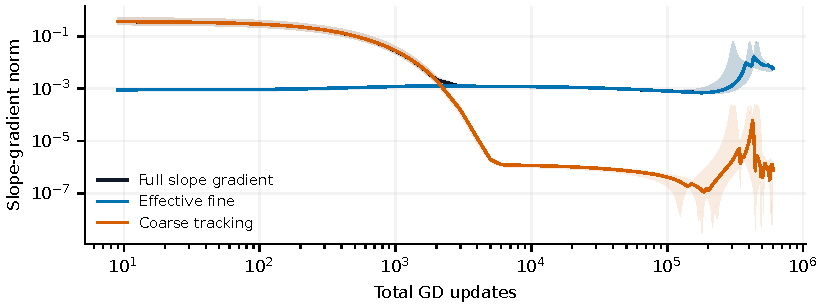
\includegraphics[width=\linewidth]{results/checkpoint_D_optimizers/expD34_readout_race/population_output/evidence/paper_latex_figures/tracking_transition.pdf}
  \caption{\textbf{Tracking loses its early dominance under GD.}
  A separate mixed-sine experiment at width 177, five seeds, and learning
  rate 0.002 over 600k updates. Curves show median slope-block norms;
  shading shows seed ranges. This full-history illustration does not
  determine the restart time for Figure~\ref{fig:scale-mechanism}. Late
  effective-force growth remains possible.}
  \label{fig:scale-tracking-transition}
\end{figure}

Figure~\ref{fig:scale-tracking-transition} uses 2,048 training inputs and
the same sine mixture normalized by training-grid RMS. Saved pre-update
coordinates end at 599,999. Every plotted coarse solve is resolved; the
numerical unresolved channel is zero. The curves are slope-block norms,
whereas Figure~\ref{fig:scale-mechanism} uses full-parameter norms to match
the force identity. A crossing of these curves is not by itself a bound
on accumulated tracking effects or a universal restart rule.

\subsection{Matched post-transient continuations}
The six-target audit uses width $W=705$, reference resolution 512,
$h=2/512$, seed 30, and 2,048 uniformly spaced midpoint inputs. Initial
slopes, hidden biases, and readouts are independent uniform draws on
$[-\sqrt{6/(W+1)},\sqrt{6/(W+1)}]$, with output bias zero; initialization
is paired across targets. All parameters train with full-batch GD at
rate 0.002. Restarts are the unmodified states after 20k updates, followed
for another 100k updates. No readout refitting or final-accuracy checkpoint
selection is used. The reference spacing normalizes scale; it does not
describe an actual grid of the learned centers.

The targets before training-grid RMS normalization are
\begin{align*}
\text{Degree five: }&0.3q_0+0.4q_1+\sqrt{0.75}\,q_5,\\
\text{Mixed sine: }&\sin(2\pi x)+0.5\sin(6\pi x)+0.25\sin(14\pi x),\\
\text{Gaussian: }&\exp\!\left(-((x+0.35)/0.22)^2\right),\\
\text{Compact bump: }&\begin{cases}\exp(1-1/(1-u^2)),&|u|<1,\\0,&|u|\ge1,\end{cases}
\quad u=(x-0.35)/0.22,\\
\text{Smooth step: }&\tanh(14(x-0.31)),\\
\text{Kink: }&|x+0.23|.
\end{align*}
Here $q_k$ are empirical orthonormal polynomials with positive leading
coefficient. The polynomial target is already normalized and is not $x^5$.
The other targets are divided by their original training-grid RMS, held
fixed thereafter. The kink and compact bump test the training mechanism
beyond the analytic target class used for the numerical construction;
the persistence theorem itself only requires $f\in L^2(\mu)$.

Effective flow uses RK4 steps 0.02 and 0.01. GD uses rates 0.002 and 0.001
over the same elapsed flow time $T=200$; the smaller-step control therefore
uses 200k updates. There are 201 saved scalar diagnostic times. These
controls test discretization sensitivity at fixed flow time; they do not
compare equal optimizer update counts.

Both panels of Figure~\ref{fig:scale-mechanism} use the smooth-step
continuation. GD tracking norm is at most 0.1963\% of effective-force norm
at saved times. The maximum relative discrepancy between GD and paired
effective-flow force norms is 0.0795\%. Trapezoidal integration of the
effective-flow rates reconstructs the log-force change with defect below
$3.16\times10^{-6}$. Integrated feedback is $0.79164$ and relaxation
contributes $-0.009283$: force grows from $0.001628$ by a factor $2.187$,
while final relative error is $0.4897$. The horizontal axes give total
training age, adding the 20k restart age to elapsed flow time divided by
0.002. This example demonstrates limited amplification with positive
reinforcement; it does not assert contraction of each slope.

\subsection{Checking the feedback condition and its usefulness}
Every target uses $B_t=4d_{\mathrm{dir}}(0)t$ in
Figures~\ref{fig:scale-feedback-force} and~\ref{fig:scale-population-error}.
Four is drawn from the tested allowance family $1,2,4,8$; coverage is an
empirical finding, not an initial-data guarantee. The largest sampled
ratio of accumulated feedback to allowance is $0.54351$.

\begin{figure}[htb]
  \centering
  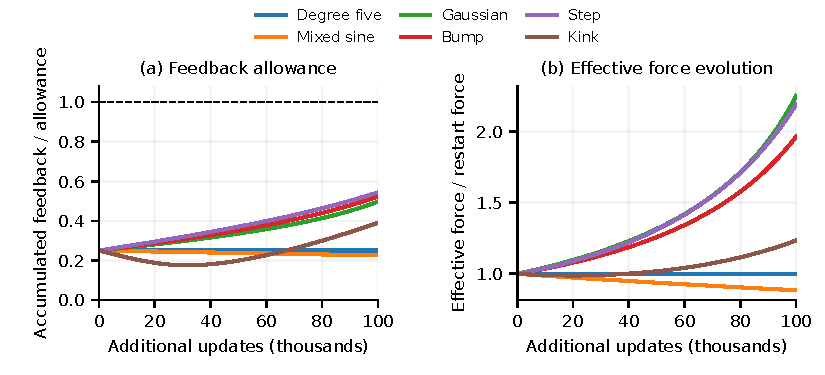
\includegraphics[width=\linewidth]{results/checkpoint_D_optimizers/expD34_readout_race/population_output/evidence/paper_latex_bounds_final/feedback_force_check.pdf}
  \caption{\textbf{The feedback condition permits either force decay or growth.}
  Six targets at width 705, from the 20k restart through 100k additional
  GD updates. Left: accumulated directional feedback divided by its common
  allowance $4d_{\mathrm{dir}}(0)t$. Right: normalized force along GD
  (solid) and effective flow (dotted). Their agreement checks the
  reduction; it is distinct from checking the feedback allowance.}
  \label{fig:scale-feedback-force}
\end{figure}

The effective-flow relative-error floors range from $0.39288$ to $0.9124$.
RMS slope-displacement allowances range from $2.51\times10^{-7}$ to
$7.74\times10^{-4}$, compared with observed GD displacements from
$2.61\times10^{-8}$ to $5.25\times10^{-5}$. For increment $0.125$, the
largest conditional ever-acquired-fraction bound is $3.84\times10^{-5}$.
All starting relative slopes are below $0.001$; this increment is already
less than needed to reach the supplied benchmark $0.25$. The independent
error floor is essential because that benchmark is not a necessary
criterion for accuracy. The lenient 1\% reference in this six-target
audit is distinct from the long Adam experiment, which passes it.

\begin{figure}[htb]
  \centering
  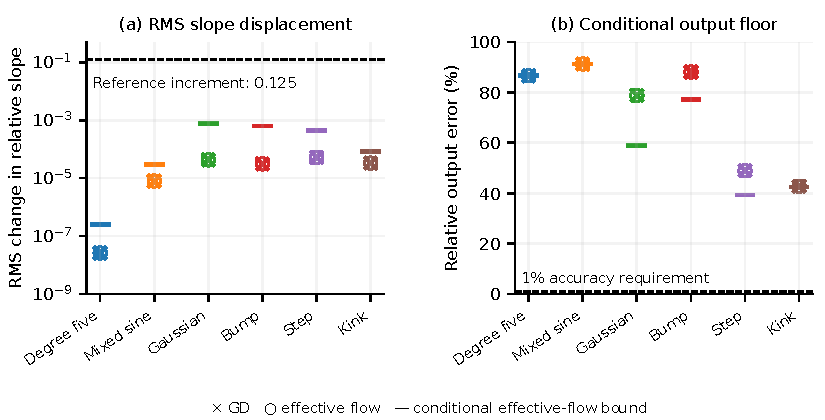
\includegraphics[width=\linewidth]{results/checkpoint_D_optimizers/expD34_readout_race/population_output/evidence/paper_latex_bounds_final/population_error_check.pdf}
  \caption{\textbf{The condition gives useful population and output bounds.}
  The same six continuations as Figure~\ref{fig:scale-feedback-force}.
  Left: endpoint RMS displacement of relative slopes, with its
  effective-flow upper bound; this is displacement from the restart,
  not the RMS level in Figure~\ref{fig:scale-observation}.
  Right: relative output errors with attached readouts and effective-flow
  lower bounds. These rounded numerical evaluations set $S=0$; GD
  agreement is measured separately. None is an interval certificate.}
  \label{fig:scale-population-error}
\end{figure}

The broader width-705 baseline contains 23 targets and two seeds, spanning
polynomial, oscillatory, localized, rational, exponential, and transition
functions. Twice the restart directional rate covers every saved prefix
of all 46 branches over 20k further updates; the largest required
multiplier is 1.367. Twelve width-1409 reference branches also pass.
These include related target variants; the six dense continuations are
part of this investigation, not six extra independent families.

Across the six targets, the largest refined GD/effective-flow endpoint
relative-error difference is $1.72\times10^{-6}$. Sampled accumulated
tracking-induced derivative loading is at most 0.0993\% of restart force.
Including sampled tracking effects in a sharper time-integrated energy
calculation changes its relative-error floor by at most $4.16\times10^{-6}$;
this is not a certified value of $\Delta_{\mathrm{err}}$
in~\eqref{eq:scale-allowances}. Halving the GD step changes endpoint
parameters by less than $1.98\times10^{-6}$ in Euclidean norm; halving
the RK4 step changes them by less than $2.4\times10^{-14}$.

The broad archive is sparse; the matched continuations are sampled densely.
Neither provides a rigorous enclosure between every saved state or for the
finite-step defect in~\eqref{eq:scale-gd-defect}. The conditional theorem
is exact, whereas verification of its premises is numerical. Force and
error use the training measure and actual attached readouts; no
continuous-input generalization or quantitative Adam guarantee is claimed.

\subsection{Empirical coverage of the population feedback loop}
The stronger theorem uses $b_0=d_{\mathrm{dir}}(0)$ and
$C(t)=2\sqrt{I_F(0)}t$. At saved prefixes, the smallest required response
coefficient is
\begin{equation}
K_{\mathrm{req}}=\max_{t_i>0}
\frac{[\mathcal B(t_i)-b_0t_i]_+}
{\int_0^{t_i}\mathcal A_4(u)\,du}.
\end{equation}
We compare it with $K_{\mathrm{crit}}=1/(e s_0G(T))$. This is a
retrospective check that useful constants exist, rather than a prediction
from the restart alone. Integrals use scalar interpolants between saved
states. The accumulated concentration allowance passes on all reported paths.

All 46 width-705 paths across 23 targets pass the sampled loop criterion
over 20k further updates; the largest $K_{\mathrm{req}}/K_{\mathrm{crit}}$
is 0.1065. All 12 width-1409 reference paths pass too. All six densely
sampled effective-flow continuations pass over that shorter duration.
At 100k further update-equivalent units, degree five, mixed sine, and kink
still pass. Gaussian, bump, and step give ratios 2.67, 3.12, and 2.24;
the broader feedback-budget bounds remain informative on all six.

For these three longer failures, the required $K$ rises only by factors
1.184, 1.131, and 1.002 compared with its first-20k estimate. The
duration-dependent sufficient criterion can therefore expire while the
response relation changes little. Doubling a coefficient fitted only on
the first 20k further updates covers the longer response on five of six
targets. Kink is the exception: its early excess feedback is zero, but
later becomes positive. These results support finite-interval response
conditions without supplying a universal extrapolation rule. Halving RK4
and GD steps preserves the pass/fail classifications. GD diagnostics test
the premises numerically; they do not certify the disturbed criterion
in~\eqref{eq:scale-loop-disturbed}.

\FloatBarrier
\section{Interventions and the domain of the mechanism}
\label{app:scale-interventions}
Function-preserving fourfold cloning divides each readout among four
identical neurons. It preserves output while dividing each copy's geometry
gradient by four and multiplying aggregate readout mobility by four.
Correcting both learning rates recovers the original trajectory to numerical
precision. Across the tested 23-target cohorts, correcting geometry mobility
largely restores slope motion, whereas correcting readout mobility alone
does not. Faster readout fitting alone is insufficient to explain this
controlled slowdown.

The smallest tested outward pulses retain 99.0--100.3\% of their directional
offset after 20k updates. This supports slow motion without strong restoration
in those tested directions, not a global attractor. Large geometry injections
can leave the weak-force regime: under the primary coarse-repair procedure,
median initial effective-force norm rises from about $6.04\times10^{-4}$
at baseline to 2.64 at 100-fold injection. The corresponding weak-force
error bound becomes uninformative; that alone does not show successful
training.

These interventions constrain the explanation without imposing one signed
force contribution across targets. Correcting generated lower-order errors
can oppose expansion, but neither universal slope contraction nor that
specific error pattern is an assumption of Theorem~\ref{thm:scale-precise}.
The claim is limited useful reinforcement over a stated interval, while
the network remains free to evolve.
